\section{MTU Discovery}
\label{sec:MTU Discovery}

\subsection{Einleitung}
Mithilfe der \acs{MTU} (Maximum Transmission Unit) wird festgelegt wie gross ein Netzwerkpaket maximal sein darf bevor es in mehrere Pakete aufgeteilt werden muss. Das finden der MTU läuft normalerweise via \acs{PMTUD} (Path MTU Discovery) ab, dabei werden \acs{ICMP} Pakete unterschiedlicher Grösse über die Verbindung gesandt und so festgestellt welches die maximale Grösse ist die noch ankommt. Das Problem dabei ist jedoch das ICMP Pakete in manchen Fällen von zu scharf konfigurierten Firewalls blockiert werden. Das heisst es kann vorkommen dass die MTU einer Verbindung nicht richtig konfiguriert ist und so kann man die Leitung nicht richtig ausnutzen. Um dieses Problem zu lösen haben wir eine \acs{MTU} Discovery Funktion im \tool entwickelt. Die Funktion verwendet ein ähnliches Vorgehen wie \acs{PMTUD}, verlässt sich dabei aber nicht auf \acs{ICMP} Pakete.
Das \tool läuft auf beiden Seiten eines \acs{IPSec} Tunnels und überwacht jeweils passiv die Verbindung. Zu in der Konfiguration festgelegten Zeitpunkten versucht jeweils eine Seite die \acs{MTU} zu ermitteln. Dabei werden laufend grössere Pakete übertragen bei denen ein "Do not fragment"-Flag gesetzt wurde. %TODO: flag verdeutschen?
So lange die Pakete auf der anderen Seite ankommen wird eine Antwort zurück gesendet. Falls keine Antwort zurück kommt weiss der Sender dass die Paketgrösse zu gross war und versucht das erneute versenden mit einer kleineren Paketgrösse.
Am Schluss wird die erfolgreich festgestellte \acs{MTU} protokolliert und die Timer beider Seiten wieder hochgestellt.

%TODO: statt Alice und 2 Alice und Bob verwenden!
\subsection{MTU-Bestimmung: Erfolgreich}
Dieses Sequenz-Diagramm stellt den idealen Ablauf bei der MTU-Bestimmung dar. Alice schickt Bob ein Paket mit dem Kommando 'MTU?'. Dieses Paket hat eine typische Grösse gem. Erfahrungswerten. Momentan starten wir mit 500Bytes. %TODO: CITATION NEEDED! GRÖSSE ANPASSEN
Bob erhält das Paket und schickt eine Antwort mit dem Kommando 'OK'. Darauf erhöht Alice
die Grösse des Pakets um einen konfigurierbaren Inkrementationswert und schickt es wieder zurück an
Bob. Dieser Ablauf wird so lange wiederholt bis das Paket nicht mehr bei Bob ankommt.
Weil das Paket nicht ankommt kann Bob keine Antwort senden und Alice läuft in ein Timeout.
Alice nimmt jetzt den letzten erfolgreichen MTU-Wert und schickt Bob erneut ein Paket.
Wenn das Paket erfolgreich ankommt, d.h. Bob ein 'OK' zurückschickt wurde die MTU erfolgreich gefunden. Alice setzt nun einen Meldung ab das die ideal MTU für die Verbindung zwischen Alice und 2 gefunden wurde.

%TODO: Grafik an aktuellen Algorithmus anpassen.

% GFX Trim left bottom right top
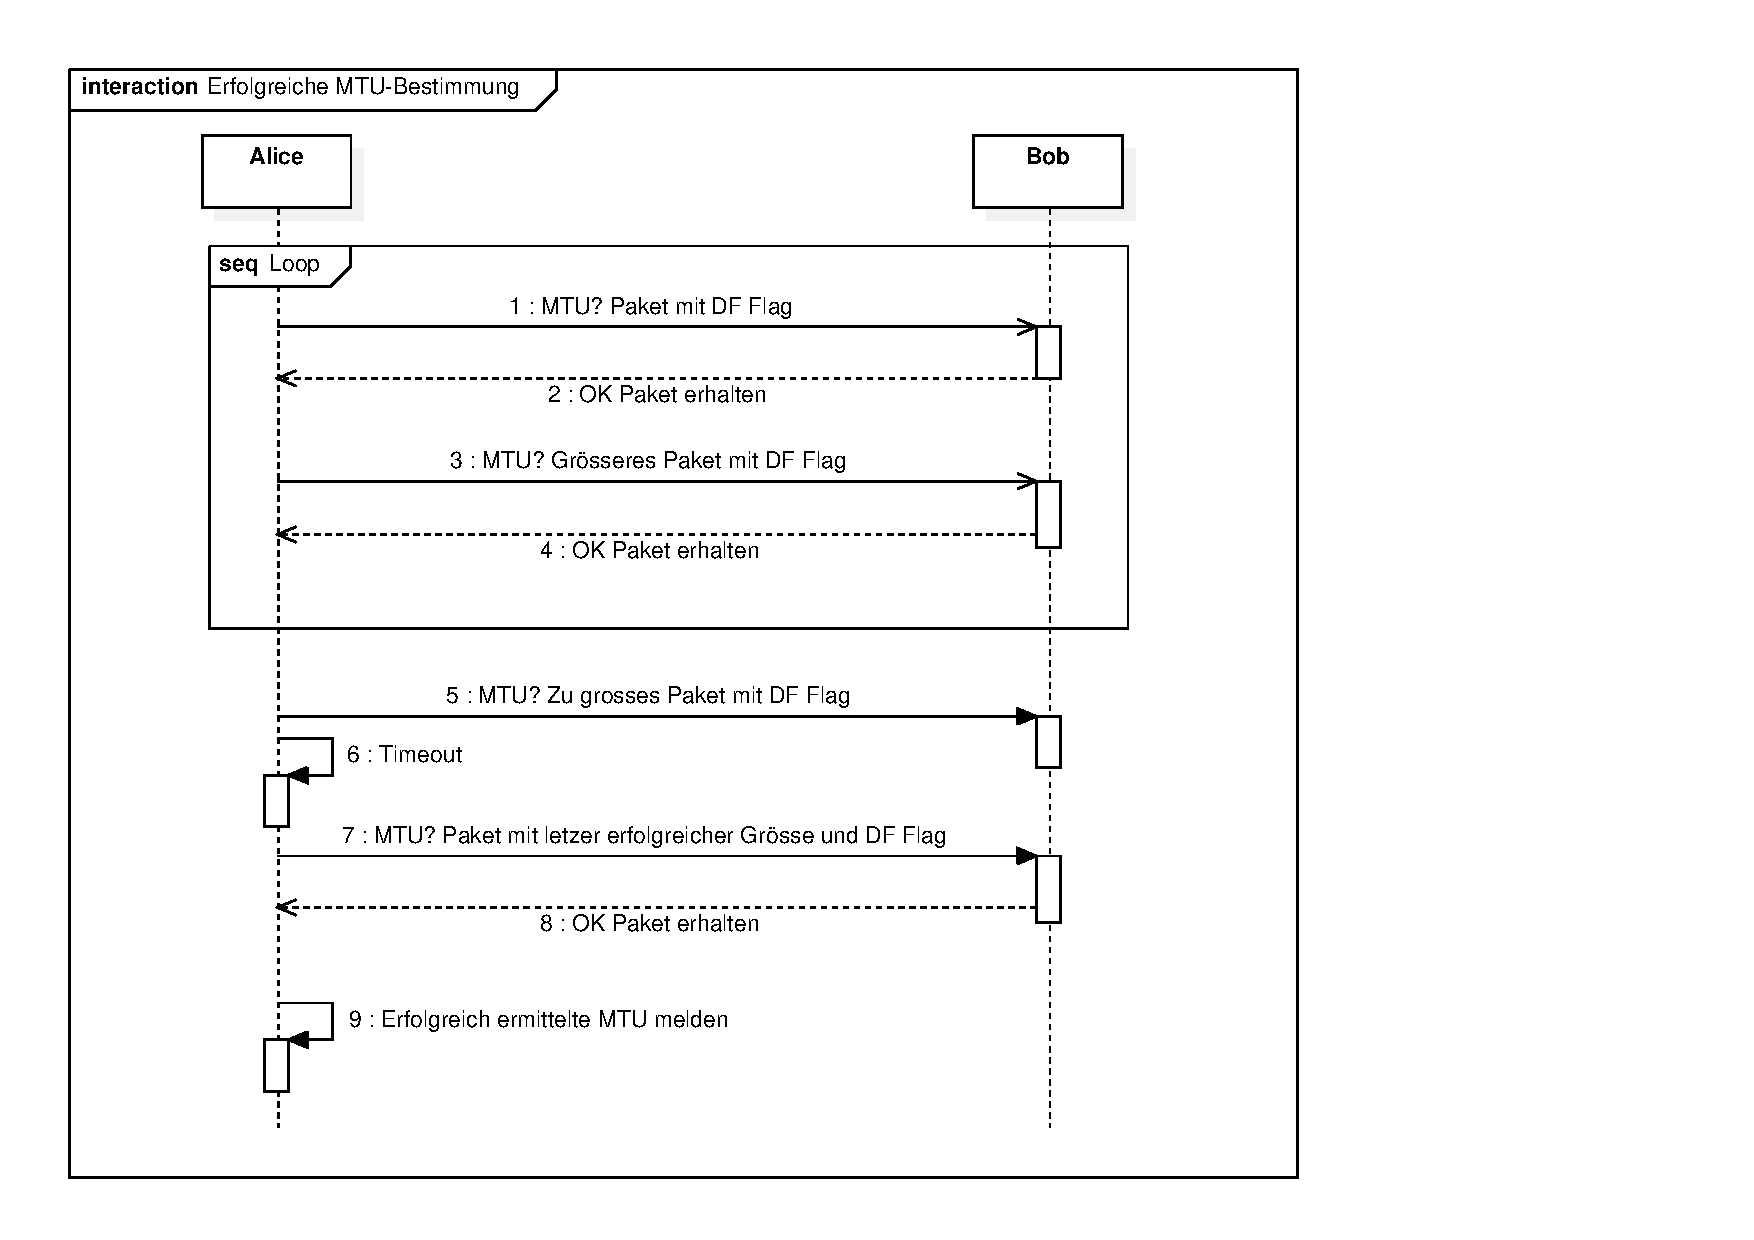
\includegraphics[trim=10 10 200 10,clip,width=\textwidth]{mainpart/implementation/img/MTUBestimmungErfolgreich}

\subsection{MTU-Bestimmung: Fehlerfall}
Dieses Sequenz-Diagramm stellt einen möglichen Fehlerfall bei der Bestimmung der MTU dar. Es zeigt wie das \tool den Fehlerfall behandelt. Alice versucht wie beim erfolgreichen Fall durch das versenden von immer grösseren Paketen die ideale MTU für die Verbindung mit Bob zu finden. Bei Punkt 5 sendet Bob keine Antwort mehr. Alice sendet Bob daher ein Paket mit der letzten erfolgreichen Grösse. Auch auf dieses Paket erhält Alice keine Antwort.  ..todo Grafik anpassen..
Schlussendliche meldet Alice die letzte erfolgreiche MTU mit einer Fehler-Nachricht und bricht den MTU Bestimmungsvorgang ab.

% GFX Trim left bottom right top
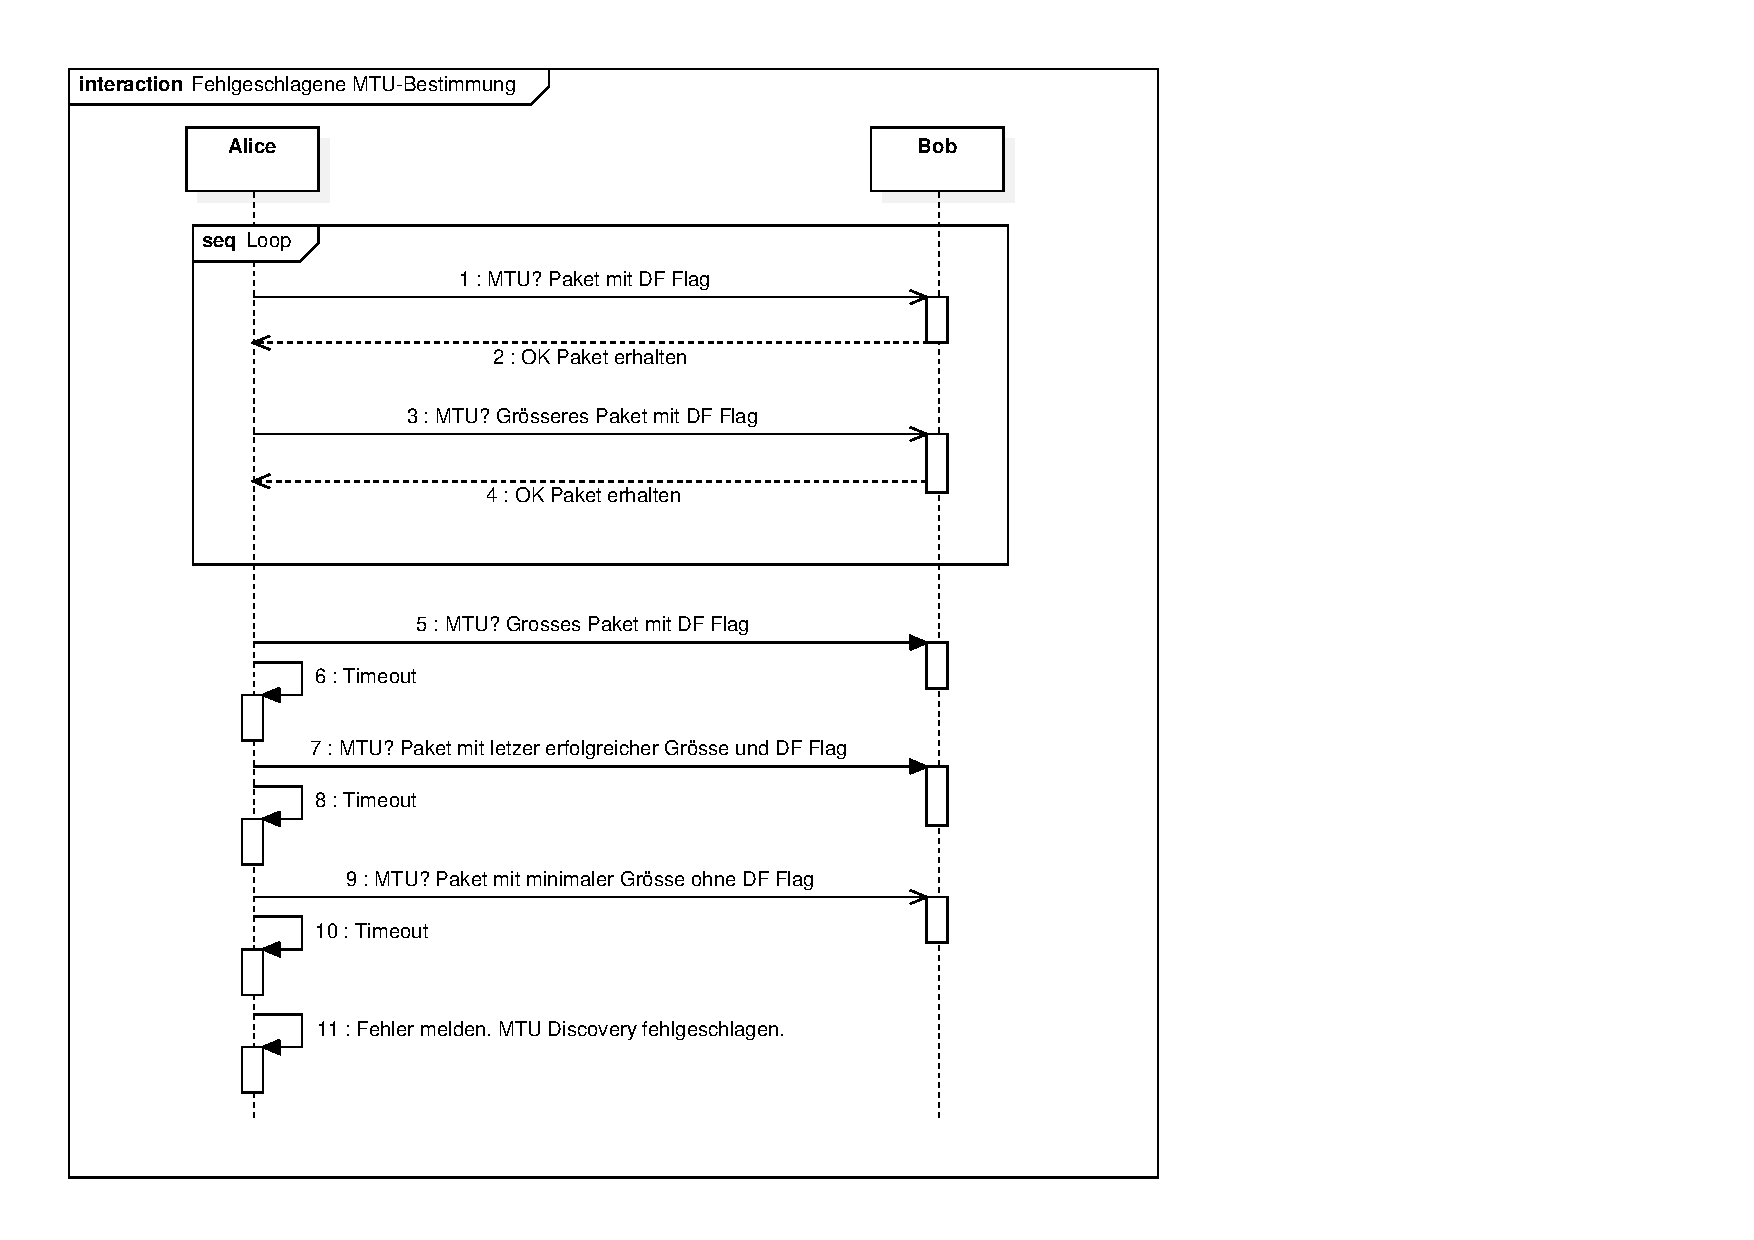
\includegraphics[trim=10 10 265 10,clip,width=\textwidth]{mainpart/implementation/img/MTUBestimmungFehlerfall}